\documentclass{beamer}
%
% Choose how your presentation looks.
%
% For more themes, color themes and font themes, see:
% http://deic.uab.es/~iblanes/beamer_gallery/index_by_theme.html
%
\mode<presentation>
{
  \usetheme{boxes}      % or try Darmstadt, Madrid, Warsaw, ...
  \usecolortheme{seahorse} % or try albatross, beaver, crane, ...
  \usefonttheme{serif}  % or try serif, structurebold, ...
  \setbeamertemplate{navigation symbols}{}
  \setbeamertemplate{caption}[numbered]
} 

%%%%%%El Señor Español%%%%%%%%%%%%%%%%%%%%%%%%%%%
\usepackage[utf8]{inputenc} %acento
\usepackage[
spanish, %El lenguaje.
es-tabla, %La tabla y no cuadro.
activeacute, %El acento.
es-nodecimaldot %Punto y no coma con separador de números
]{babel}

\usepackage[utf8]{inputenc}
\usepackage[T1]{fontenc}
\usepackage{nicefrac}

\title[Avance]{Acerca de la tesis de maestría\\(hasta ahora)}
\author{Evelyn Coronel}
\institute{Partículas y Campos - Centro Atómico Bariloche}
%\date{Date of Presentation}

\begin{document}

\begin{frame}
  \titlepage
\end{frame}

% Uncomment these lines for an automatically generated outline.
%\begin{frame}{Outline}
%  \tableofcontents
%\end{frame}

\section{Introducción}

\begin{frame}{Introducción}

\begin{itemize}
  \item Cosas que hice en la tesis de licenciatura.
  \begin{itemize}
  	\item[-] Corrección del clima
  	\item[-] Familiarizarse con el dataset
  \end{itemize}
  \item Resultados a los que llegué.
  \item Nos movimos a otros disparos (MoP y ToTs)
\end{itemize}

\end{frame}

\begin{frame}{Introducción}

\begin{figure}[htbp]
  \centering
  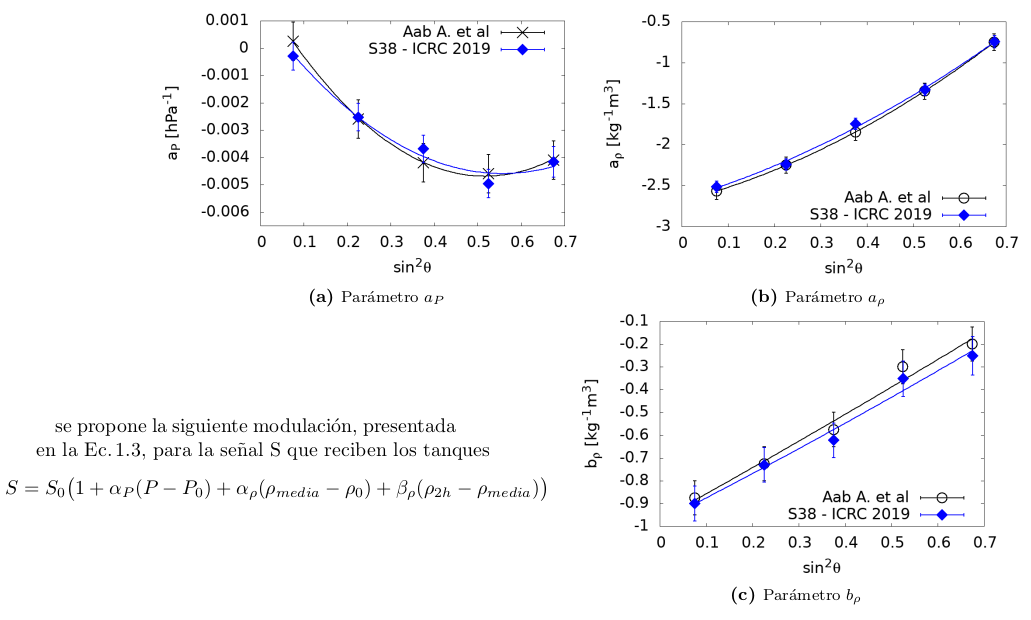
\includegraphics[width=0.95\textwidth]{tesis.png}
\end{figure}

\end{frame}

\section{Update}

\begin{frame}{Update}

  \begin{itemize}
  	\item Diferencias con el disparo tradicional.
    \begin{itemize}
      \item[-] Empieza en el 2013
      \item[-] Eficiencia
      \item[-] Cantidad de datos en el bin de 1 EeV - 2 EeV.
    \end{itemize}
  	\item Pesos de los hexágonos.
  	\item Resultados con el rango de energía 1 EeV - 2 EeV.
    \item ¿Podemos mejorarlo con la corrección del clima?
  \end{itemize}


\end{frame}


\subsection{Cálculo de Rayleigh.}

\begin{frame}{Pesos}
\frametitle{Cálculo de Rayleigh: ¿Por qué importan los pesos?}

 \begin{enumerate}
   \item Fijo una frecuencia a estudiar.
   \item Me muevo en el dataset de hexagonos, a cada utc lo clasifico según:
   \begin{equation*}
     h = (\text{hora local })\times \nicefrac{\text{Frecuencia a estudiar}}{\text{Frecuencia Solar}}
   \end{equation*}
     \item El valor de h no es continuo, sino está divido en 288 segmentos entre 1 y 24
  \item Le asigno un peso al bin h:
   \begin{align*}
     \text{peso del bin h} &= \nicefrac{\text{Hexagonos que cayeron en el bin h}}{I}\\
     I &= \sum^{288}_h \nicefrac{\text{Hexagonos que cayeron en el bin h}}{288}
    \end{align*} 

 \end{enumerate}

\end{frame}



\subsection{Pesos de los hexágonos}

\begin{frame}{Pesos}
\frametitle{Pesos de los hexágonos}

\begin{figure}[htbp]
  \centering
  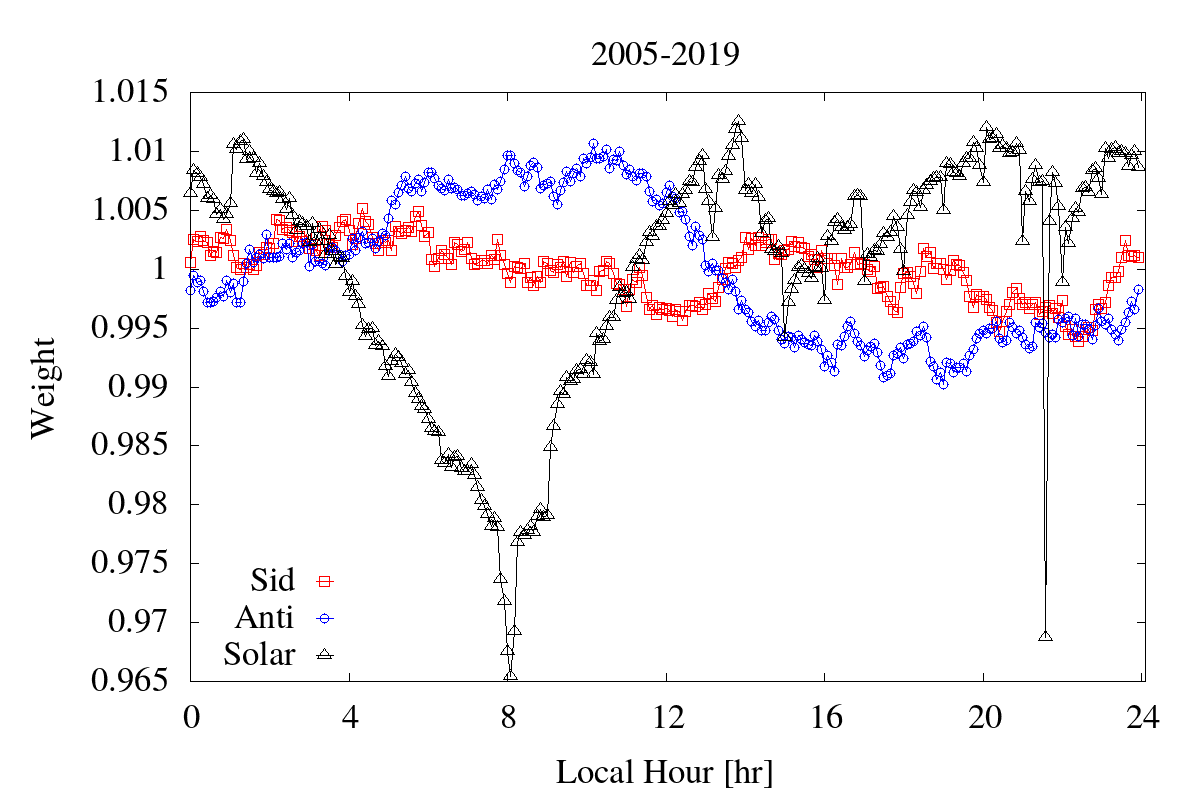
\includegraphics[width=0.95\textwidth]{./../../Cpp/Anisotropy/report_2_27_04_2020/weigth2005-2019.png}
  \caption{Un ejemplo de pesos de los hexágonos en el rango 2005-2019 para distintas frecuencias.}
\end{figure}

\end{frame}

\begin{frame}{Pesos}
\frametitle{Pesos de los hexágonos}

\begin{figure}[htbp]
  \centering
  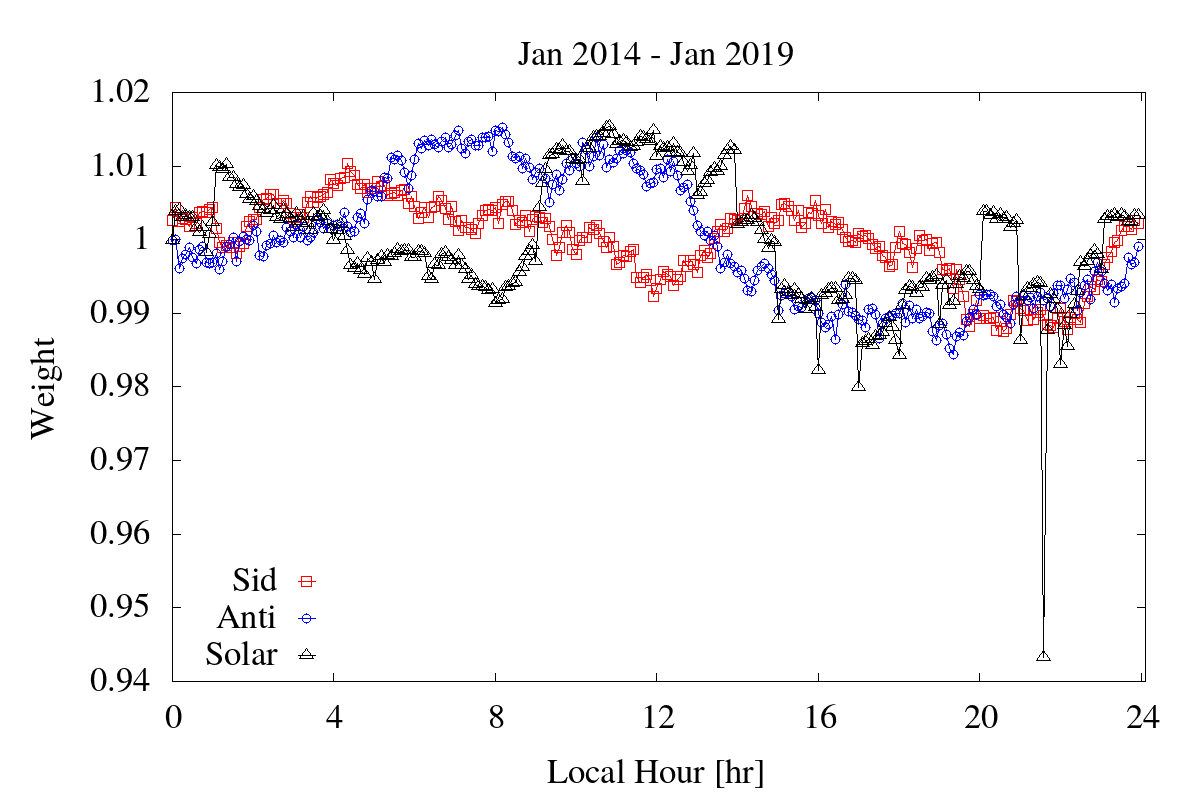
\includegraphics[width=0.95\textwidth]{./../../Plotting/weigth2014-2019_jan.png}
  \caption{Un ejemplo de pesos de los hexágonos en el rango Enero 2014- Enero 2019 para distintas frecuencias.}
\end{figure}

\end{frame}



\subsection{Cálculo de Rayleigh.}

\begin{frame}{Pesos}
\frametitle{Cálculo de Rayleigh: ¿Por qué importan los pesos?}

 \begin{enumerate}
   \item Fijo una frecuencia a estudiar.
   \item Me muevo en el cielo con esa frecuencia (fase).
   \item Dado el utc del evento, lo clasifico según:
   \begin{equation*}
     h = (\text{hora local })\times \nicefrac{\text{Frecuencia a estudiar}}{\text{Frecuencia Solar}}
   \end{equation*}
     \item El valor de h no es continuo, sino está divido en 288 segmentos entre 1 y 24
  \item Le asigno un peso por evento:
   \begin{equation*}
     \text{peso del evento} = (\text{peso  de los hexágonos para el bin h})^{-1}
     \end{equation*} 
    \item Hago el análisis en frecuencias:
    \begin{align*}
        a &= \sum^{Eventos}_i \cos(2\pi \nicefrac{h}{24} + (RA -RA_{cenit}))\times \nicefrac{(\text{peso del evento})_i}{N}\\
        b &= \text{Lo mismo pero con seno}\qquad         N = \sum^{Eventos}_i \text{peso del evento}_i
    \end{align*}
 \end{enumerate}

\end{frame}



\subsection{Resultados con el rango de energía 1 EeV - 2 EeV}


\begin{frame}{Bin 1EeV-2EeV}
\frametitle{Resultados con el rango de energía 1 EeV - 2 EeV}

\begin{figure}[htbp]
  \centering
  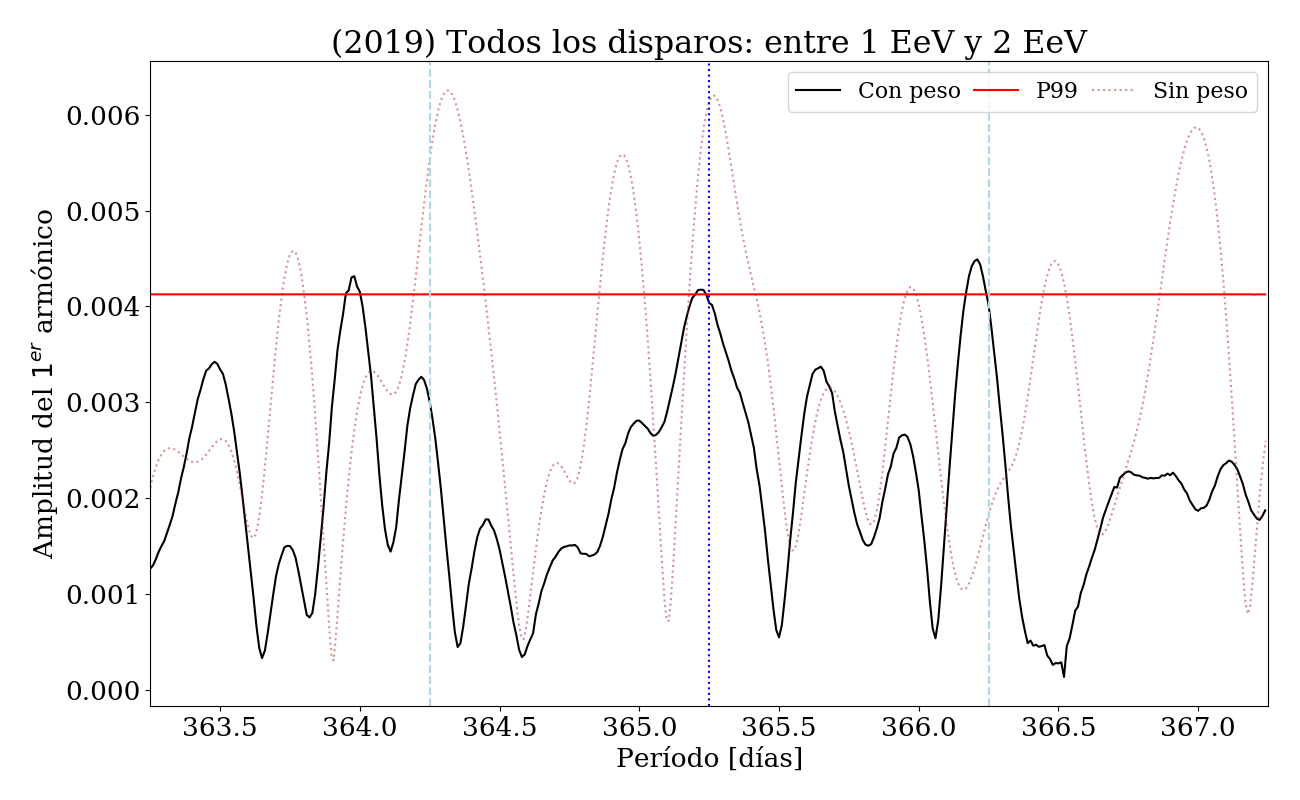
\includegraphics[width=\textwidth]{./../../Python/xx2019_AllTriggers_1_2_EeV_con_vs_sin_peso.png}
  \caption{Análisis en frecuencia para el bin 1 EeV - 2 EeV, entre Enero 2014- Enero 2019 (Cantidad de eventos $ \approx 10^6$).}
\end{figure}

\end{frame}





\end{document}